% Chapter 1
\chapter*{Introduction}
\label{chap:introduction}

The work presented in this thesis is centered around the design, development, and testing of an astronomical balloon-borne telescope called BETTII: the Balloon Experimental Twin Telescope for Infrared Interferometry. Developed at NASA Goddard Space Flight Center, this instrument is exploring a new observation technique called "Double-Fourier" interferometry, which could lead to future space-borne telescopes with very high angular resolution in the far-infrared regime. Various fields in astronomy would benefit from such enhanced capability, as demonstrated by the success of far-infrared single-aperture telescopes such as \WISE, \Spitzer and \Herschel. 

More than just a pathfinder, BETTII is a scientific instrument in its own right. For its first flights, it will study regions of clustered star formation with unprecedented details, providing almost an order of magnitude better spatial resolution than any existing or past far-IR facility.

This thesis describes some aspects of my involvement with BETTII as well as my contributions to the scientific field of clustered star formation using the only existing far-IR facility, SOFIA. The document is organized as follows:
\begin{itemize}
\item Chapter~\ref{chap:StarFormation} describes the framework and current understanding of how stars are forming in clusters, and lays out the key tools that we use to study these regions.
\item Chapter~\ref{chap:SOFIA} is a study of nearby star-forming clusters using new data that we obtained with the SOFIA observatory. SOFIA offers moderately high angular resolution, which we attempt to use to improve the study of the brightest, densest regions of star formation. This work is to be submitted for publication shortly after the conclusion of this dissertation. 
\item Chapter~\ref{chap:BETTII} describes the physical principles of interferometry which drive the design of the balloon instrument. We discuss how sensitive the instrument will be and identify scientific targets and calibrators that are suitable for our first flights.
\item Chapter~\ref{chap:phasenoisepaper} is a standalone, refereed publication that was published in 2015 on the spectral sensitivity of double-Fourier interferometers in general. It proposes a mathematical framework to analyze the sensitivity of such instruments to various types of noise sources. We apply those findings to the case of BETTII.
\item Chapter~\ref{chap:controls} discusses the design of the control system for BETTII, which presents unique challenges compared to any other balloon-borne instrument. We also discuss the controls algorithm that is used in flight to properly estimate the orientation of the payload, a key requirement to achieve successful interferometry.
\item Chapter~\ref{chap:implementation} shows results of the implementation that we discusses in the previous chapter. This consists of laboratory and on-sky testing of the observatory. We discuss the expected performance at float.
\item Chapter~\ref{chap:conclusion} summarizes our findings and discusses the path forward for the BETTII project.
\end{itemize}


\chapter{Star formation in clustered environments} % Main chapter title

\label{chap:StarFormation}

%----------------------------------------------------------------------------------------


\section{Molecular Clouds}

Molecular clouds are the dense regions of the interstellar medium (ISM) where stars are forming. They contain about half the mass of the ISM in $<2$\% of its volume \citep{Ferriere:2001gv}. High densities ($n > \SI{100}{\centi\meter\raiseto{-3}}$) of mostly molecular hydrogen and low temperatures ($< \SI{20}{\kelvin}$) distinguish molecular clouds from the various other components of the ISM in galaxies: the Warm Neutral Medium (WNM), the Warm Ionized Medium (WIM), and the other cold phase of the ISM, the Cold Neutral Medium (CNM), which is thought to be the parent region in which molecular clouds are formed \citep{Kennicutt:2012ey}. In addition to molecular hydrogen, molecular clouds also contain Helium (10\% by number), dust ($\sim 1\%$ by mass), CO ($\sim \num{1e-4}$ by number), and traces of many other molecules.

Observations of molecular clouds reveal that they are highly structured with often a filamentary pattern [cite shaye?]. While the literature proposes multiple classifications for the various structures found in molecular clouds, we choose to focus only on two structures which are key to this work: clusters, which are more local associations of stars in virial equilibrium \citep{Lada:2003il}; and dense cores, which are sites where stars form individually or in systems of small multiples \citep{Williams:2000wl}. Clusters are formed of multiple cores, but cores can also be found outside of clusters, in the field. In the classical picture, clouds are thought to fragment into clusters, which still contain many times the Jeans' mass - the minimum mass for gravitationally-bound cores \citep{Larson:1994cj} which are also called prestellar cores \citep{DiFrancesco:2007vg}.

%[The structure of clusters itself is of great interest to study the mechanisms at stake in star formation, because it gives information about the cluster's origins \citep{Lada:2003il}. Clusters are believed to be relatively short-lived, because the stars it forms can disrupt its gravitational equilibrium. Typical timescales for clusters are on the order of \SI{100}{\mega\year} \citep{Lada:2003il}. ]

Approximately 60\% of all stars are thought to form in embedded, young stellar clusters of 1-\SI{3}{\mega\year} with 100 or more stars \citep{Porras:2003kxa,Allen:2007wqa}. These $>$100 star clusters have characteristic sizes of 2-4 parsecs (pc) with peak surface densities of 100-\si{1000} stars per square parsec and a typical median distance between nearest neighbor young stellar objects (YSOs) of 0.03 to 0.06 pc \citep{Gutermuth:2009gca}.

Because star-forming clusters are surrounded by interstellar matter from the parent molecular cloud, they usually cannot be studied at optical wavelengths, due to the large obscuration from dust grains along the line of sight. Infrared observations can be used to probe these structures since the dust can acquire sufficient temperature to emit thermally from the mid-infrared to millimeter and radio wavelengths. 

The high density of YSOs within clusters, combined with their typical separations of few hundredths of parsecs requires a high angular resolution in order to capture the relevant spatial scales at which accretion mechanisms are occurring to give the star its final mass.




\section{Star formation}

\subsection{Standard models}

A considerable amount of literature exists on star formation and the various physical processes involved in forming stars. In this section, we review some of the most standard views that describe how stars are born and grow to acquire their final masses.

\subsubsection{Gravitational collapse}

A simple way to derive characteristic quantities related to the formation of stars is to consider a pre-stellar core as a spherical clump of uniform, isothermal gas in hydrostatic equilibrium. For such a system, the Virial theorem applies, which describes the balance between the gravitational potential and the kinetic thermal energy within the gas. In other words, in hydrostatic equilibrium, the core's self-gravity is compensated by the internal pressure caused by the temperature of the gas. For the same radius and temperature, a core with more mass will lead to a runaway collapse. While simplistic, this treatment leads to a handy derivation of critical timescales, sizes, and masses that form a good starting point for more elaborate theories. 

First, it is important to determine what are the characteristic timescales of star formation. In the core with a uniform density, the simplest timescale to define is called the free-fall time: this is the time it takes for the total gravitational collapse of a spherically-symmetric clump of uniform density $\rho$ if only the force of gravity is considered:
\begin{equation}
\tff \sim \left(\frac{3\pi}{32 G\rho}\right)^{-1/2}\sim \SI{2e5}{\year}\left(\frac{\rho}{\SI{e-19}{\gram\per\raiseto{3}\centi\meter}}\right)^{-1/2},
\end{equation}
where we have substituted a typical value for the gas density in clusters. The free-fall time is usually a lower limit on the collapse timescale, since there will always be some thermal pressure that will resist gravity and slow down the infall of gas into the potential well. 

The other relevant quantity that involves time is the sound speed in the cloud, $\cs = (kT/(\mu m_H))^{1/2}$, where $\mu$ is the mean molecular weight of the gas and $m_H$ the mass of hydrogen. For a given spatial scale $R$, the sound-crossing time is defined as $\ts = R/\cs = \SI{4.9e5}{\year}\left(\frac{R}{\SI{0.1}{\pc}}\right)\left(\frac{\cs}{\SI{0.2}{\kilo\meter\per\second}}\right)^{-1}$. This is the time it takes for a wave to cross the scale $R$ while traveling at the sound speed.
Intuitively, if the core has a size $R$ such that $\tff<\ts$, it will tend to collapse faster the gas in the cloud can compensate to maintain hydrostatic equilibrium. This corresponds to a characteristic sizescale that is called the Jeans' length, and corresponds to the characteristic sizescale of gravitational instability within a cloud \citep{McKee:2007bd}:
\begin{equation}
 \lambdaJ = \cs\times\tff = \SI{0.04}{\pc}\left(\frac{\cs}{\SI{0.2}{\kilo\meter\per\second}}\right)\left(\frac{\rho}{\SI{e-19}{\gram\per\raiseto{3}\centi\meter}}\right)^{-1/2}.
 \end{equation} 

The Jeans mass is the amount of mass within a sphere of diameter \lambdaJ, and corresponds intuitively to the minimum mass a core needs to gather in order to trigger an gravitational collapse:
\begin{eqnarray}
\MJ &=& \frac{4\pi}{3}\rho\left(\frac{\lambdaJ}{2}\right)^3 \\
&=& \SI{0.06}{\Msun} \left(\frac{\cs}{\SI{0.2}{\kilo\meter\per\second}}\right)^3 \left(\frac{\rho}{\SI{e-19}{\gram\per\raiseto{3}\centi\meter}}\right)^{-1/2}
\end{eqnarray}

Note that this formalism completely ignores the material that surrounds the core while it collapses. In practice, the cloud exerts an external pressure on the core that needs to be taken into account when calculating the critical masses. This more elaborate case of a clump of self-gravitating gas on the verge of collapse that is immersed in a medium of external pressure $\Pext$ is called a Bonnor-Ebert sphere. It can be shown \citep{McKee:2007bd} that the sizescale is similar to the Jeans' length, and the mass scale is a few times smaller than the Jeans' mass, which stays well within the accuracy limits of our simple model.

Once the gas starts its gravitational collapse, nothing stops it until the central pressure and density reach values that trigger the ignition of nuclear fusion. This is the birth of the star. This new mechanism creates a large amount of radiation pressure that balances out the collapse and forms a new hydrostatic equilibrium. 

In practice, it is likely that a single core fragments into multiple centers of collapse, each of them exceeding the local Jeans mass. This would create systems of binaries or small multiples instead of single stars, a scenario that is currently favored [LARSON?].

In the standard model, the collapse begins at the center of the core and propagates outward at the sound speed, so the density structure of the initial core will change as a function of time. Most models result in an infalling envelope with density profiles which follow power laws from $\renv^{-1.5}$ to $\renv^{-2}$, an important observable that can be useful to test these theories. Some models of slowly-rotating infalling clouds suggest more complex density profiles for the envelopes \citep[e.g.][]{Ulrich:1976ho,Terebey:1984hi} than simple power laws, but are observationally difficult to constrain due to the small differences with traditional power-law envelopes and the small scales at which those differences occur (a few 100's of AU).

Through conservation of angular momentum, some of the surrounding material naturally flattens into a centrifugally-supported flaring disk before it is fed to the star, and a bipolar cavity opens along the rotation axis of the system. The cavity opening can also be bolstered by mechanisms such as stellar winds and jets [REFERENCE].

The object now has three characteristic components: the star itself; the flattened disk; and a diffuse envelope with an open cavity, which constitutes a mass reservoir for future accretion onto the star.

The accretion rate represents the speed at which the mass is transferred between different objects, and are important to set relevant timescales and to relate observables to the physics. For relatively low-mass star formation, the usually adopted accretion mechanism is called Shu accretion \citep{Shu:1977ef}, and predicts a mass accretion rate of the envelope onto the disk $\Mdotenv \propto \cs^3/G$, where $\cs$ here represents the sound speed that includes turbulence, and $G$ is the gravitational constant. Typical accretion rates for $\cs\sim \SI{2.7}{\kilo\meter\per\second}$ are $\Mdotenv \sim  \SI{4.8e-6}{\Msun\per\year}$ \citep{Dunham:2010bx}.

Although most of the mass is contained in the $\textrm{H}_2$ gas, there is a small fraction of material in the form of dust grains of various sizes and populations. Despite their low mass, these grains play a very important role in determining the observable properties of YSOs, because of their tendency to absorb short wavelengths and radiate in the thermal infrared (see Section~\ref{subsec:dust}). 

%The accretion mechanism most commonly consists of Bondi accretion \citep{Bondi:1952fc}, and represents the transfer of mass from the envelope or the disk to the star. As the YSO moves through its parent cloud, it can also accrete more mass throughout its life that was not originally part of the original condensation that initiated the collapse. In these dense regions where multiple stars are forming, interactions between YSOs is more than likely and can significantly affect the final masses of stars.

%Various models exist for accretion, from a quasi-static slow process \citep{Shu:1977ef} to a very rapid and brutal process \citep[e.g.][]{Larson:1967ee}. \cite{McKee:2007bd} suggest that the infall process is most likely slowing down as a function of time, which complicates its observational validation. 


% , the speed of sound is $c_s = (kT/m)^{1/2}$.
%Perhaps the most elementary way to model the birth of a star consists of considering an isothermal sphere of self-gravitating gas (a core) on the verge of collapse, in hydrostatic equilibrium with its surrounding cloud medium of gas pressure \Pext. This is also called a Bonnor-Ebert sphere \citep{Ebert:1955wf,Bonnor:1956cy}, and the state of this sphere is said to be \textit{critically stable}, with a critical mass defined by $\Mcrit = 1.18\frac{c^4_s}{G^{3/2}}\Pext^{-1/2}$ \citep{Shu:1977ef}, where $c_s = (kT/m)^{1/2}$ is the speed of sound in the cloud. To put this in perspective using physical quantities, we have:
%\begin{equation}
%M_{BE} = 0.66 \left(\frac{T}{\SI{10}{\kelvin}}\right)^2 \left(\frac{\Pext/k_B}{\SI{3e-5}{\raiseto{-3}\centi\meter\kelvin}}\right)^{-1/2}\si{\Msun},
%\end{equation}
%where \Pext was normalized to mean kinetic pressure at the surface of molecular clouds \citep{McKee:2007bd}. The Bonnor-Ebert radius is $R_{BE} = 0.49 c_s/(G\rho_0)^{1/2}$,  which is comparable to the characteristic fragmentation size scale called the Jeans' length. Here $\rho_0$ is the uniform density of the core. 

%For a core of mass $M_{BE}$, the thermal pressure exactly compensates the gravitational forces. Collapse occurs for cores with mass $>M_{BE}$ when gravity overcomes the thermal pressure of the gas inside the sphere, which triggers the rapid mass growth of a central embryo towards infinitely high densities. In practice, the process stops when enough density is reached to ignite nuclear fusion and stabilize the embryo, which has just become a young stellar object. Even after the star is born, mass continues to fall into the potential well, emitting radiation and increasing the mass of the central object. Various scenarios exist for this phase of the accretion within individual cores, 




%Since the accretion rate can be linked to the observed luminosities as gas falls into the gravitational potential well, it is also an important outcome of a given collapse model.
%For low-mass star formation from cores that are marginally super-critical, the infall phase can be treated in the quasi-static limit \cite{Shu:1977ef} and follows this normalized form \citep[Eq.44,][]{McKee:2007bd}:
%\begin{equation}
%\dot{m}_{infall} = \num{1.54e-6} \left(\frac{T}{\SI{10}{\kelvin}}\right)^{3/2}\si{\Msun\per\year}.
%\end{equation}

%More massive stars follow an accretion behavior more similar to Bondi-Hoyle accretion
%Conserving its original angular momentum

%[Accretion rates are likely varying as a function of time {McKee:2007bd}, and can complicate the interpretation ]

%[Magnetic fields, turbulence, asymmetries and non-isothermal considerations all likely play role in this balance, but dramatically complicate the mathematical treatment of the problem. In order to introduce the basic concepts of star formation, these complex processes are ignored.]

%\citep{Myers:2014ct}; includes why accretion stops. Shu accretion for low mass, Bondi accretion at high mass?

\subsubsection{YSO classification and characteristics}

We have determined that YSOs are composed of a star, a disk, and an envelope. The star is believed to be fairly well understood as a young object in hydrostatic equilibrium on its way to the main sequence. Depending on many parameters, the spatial distribution of gas in the disk and the envelope can be predicted by simple models, but in all likelihood is very complex, inhomogeneous, and asymmetric. 
%Often, the envelope is thought to open up a cavity around the poles of the rotating system, where material can escape the system (through outflows, for example [REFERENCE?]). 
For clarity, we will discuss here the simple models that can be used to describe the YSOs in the multiple stages of their evolution.

In the most common model of the evolution of young stars, there are four stages in the lifetime of a YSO. The first stage consists of a dense core right after the YSO is born. The disk is almost inexistent, the envelope still is dense and circularly symmetric. This is called Stage 0. As the system evolves, the cavity opening angle grows, the density of the envelope decreases, and the size of the disk increases. When a YSO is Stage III, both the disk and the envelope are almost entirely depleted.

The various stages of YSO (from 0 to III) have very distinct observational signatures, although are highly dependent on the viewing angle. The most commonly used tool to classify YSOs based on their SEDs is to use the spectral index, which corresponds to the mid-IR slope $\alpha$ in the log-log plots, with $\alpha = \textrm{d}(\lambda F_\lambda)/\textrm{d}\lambda$ between 2 to \SI{20}{\micro\meter} \citep{McKee:2007bd}. The four classes of YSOs are:


\begin{figure}[!h]
\begin{center}
\subcaptionbox{Stage 0\label{subfig:Stage0}}{
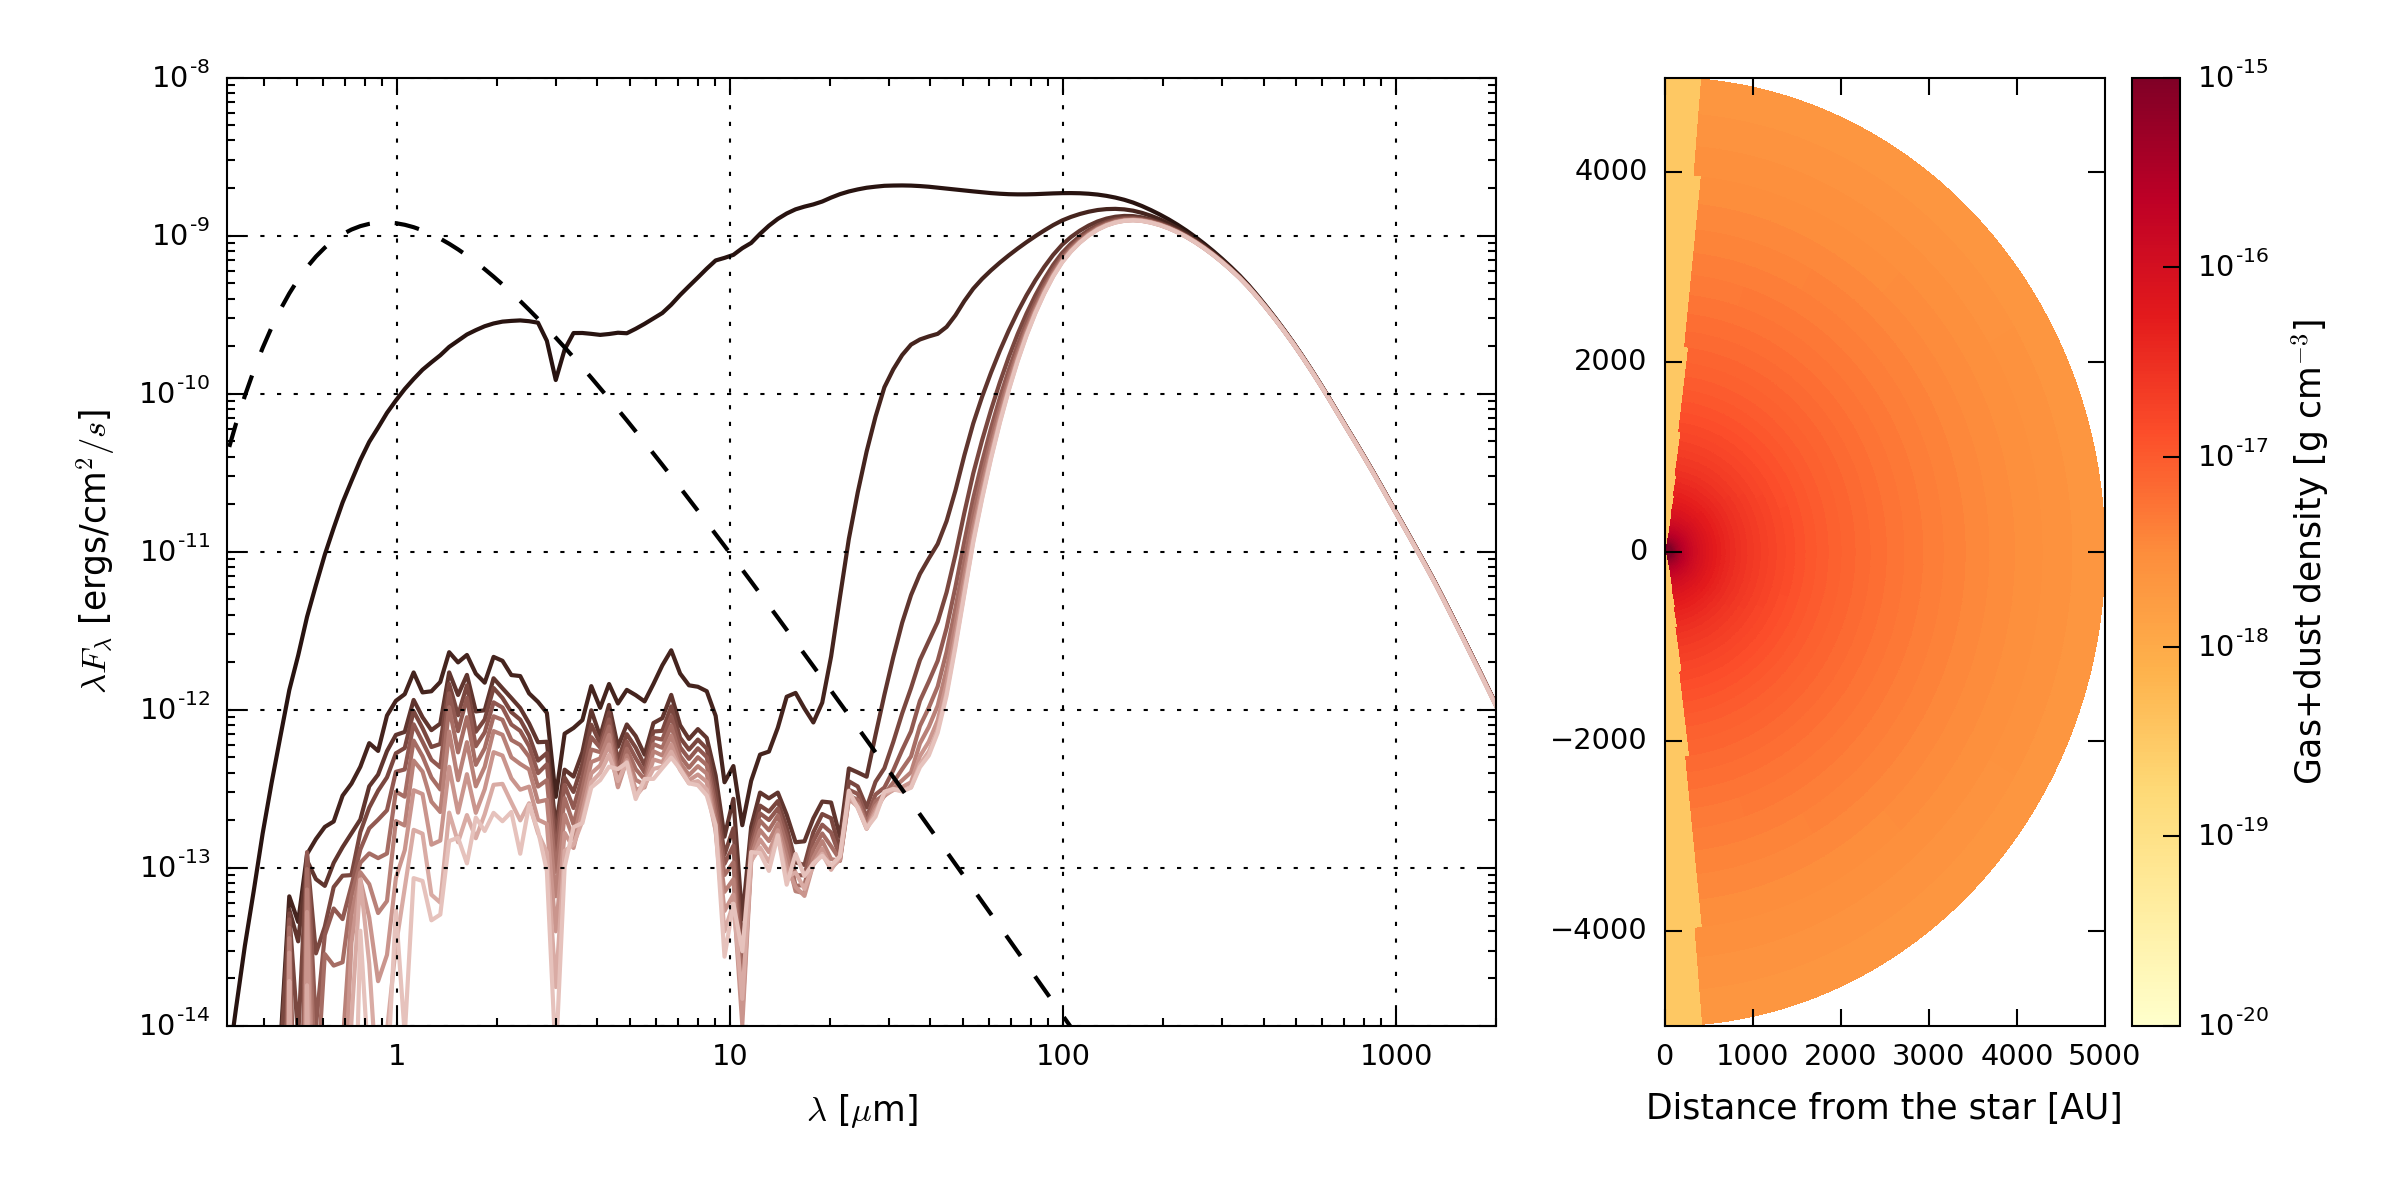
\includegraphics[width=\textwidth]{Figures/test_whitney_class0_nice.png} 
} \par\medskip
\subcaptionbox{Stage I.\label{subfig:StageI}}{
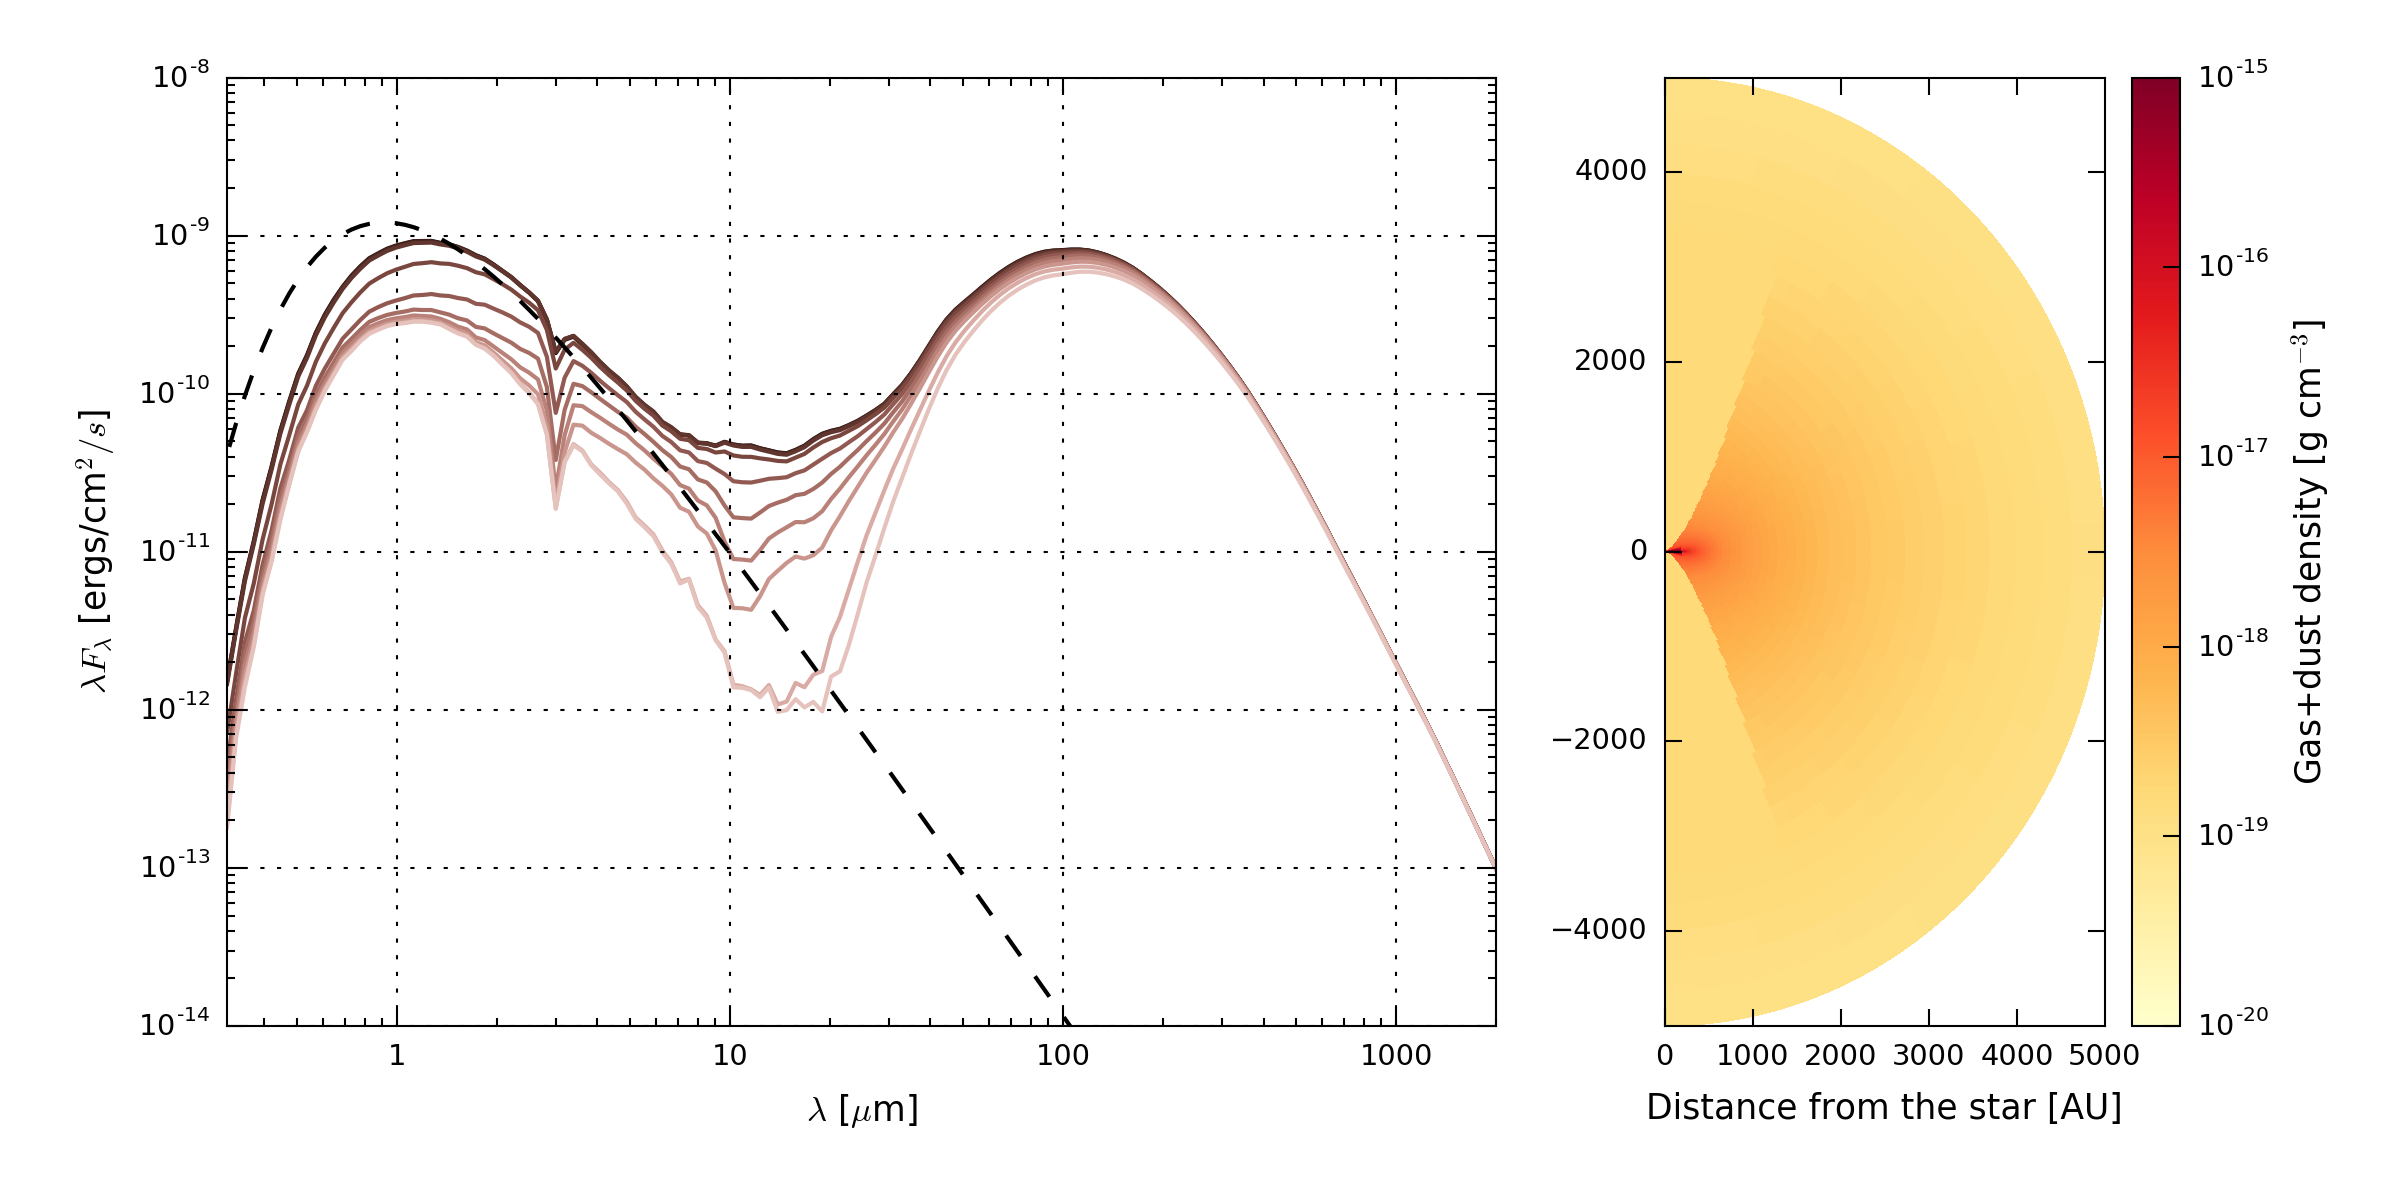
\includegraphics[width=\textwidth]{Figures/test_whitney_classI_nice.png} 
} 
\caption[Early evolution of YSOs]{Early evolution of YSOs.}
\label{fig:EarlyStages}
\end{center}
\end{figure}

\begin{figure}
\begin{center}

\subcaptionbox{Stage II.\label{subfig:StageII}}{
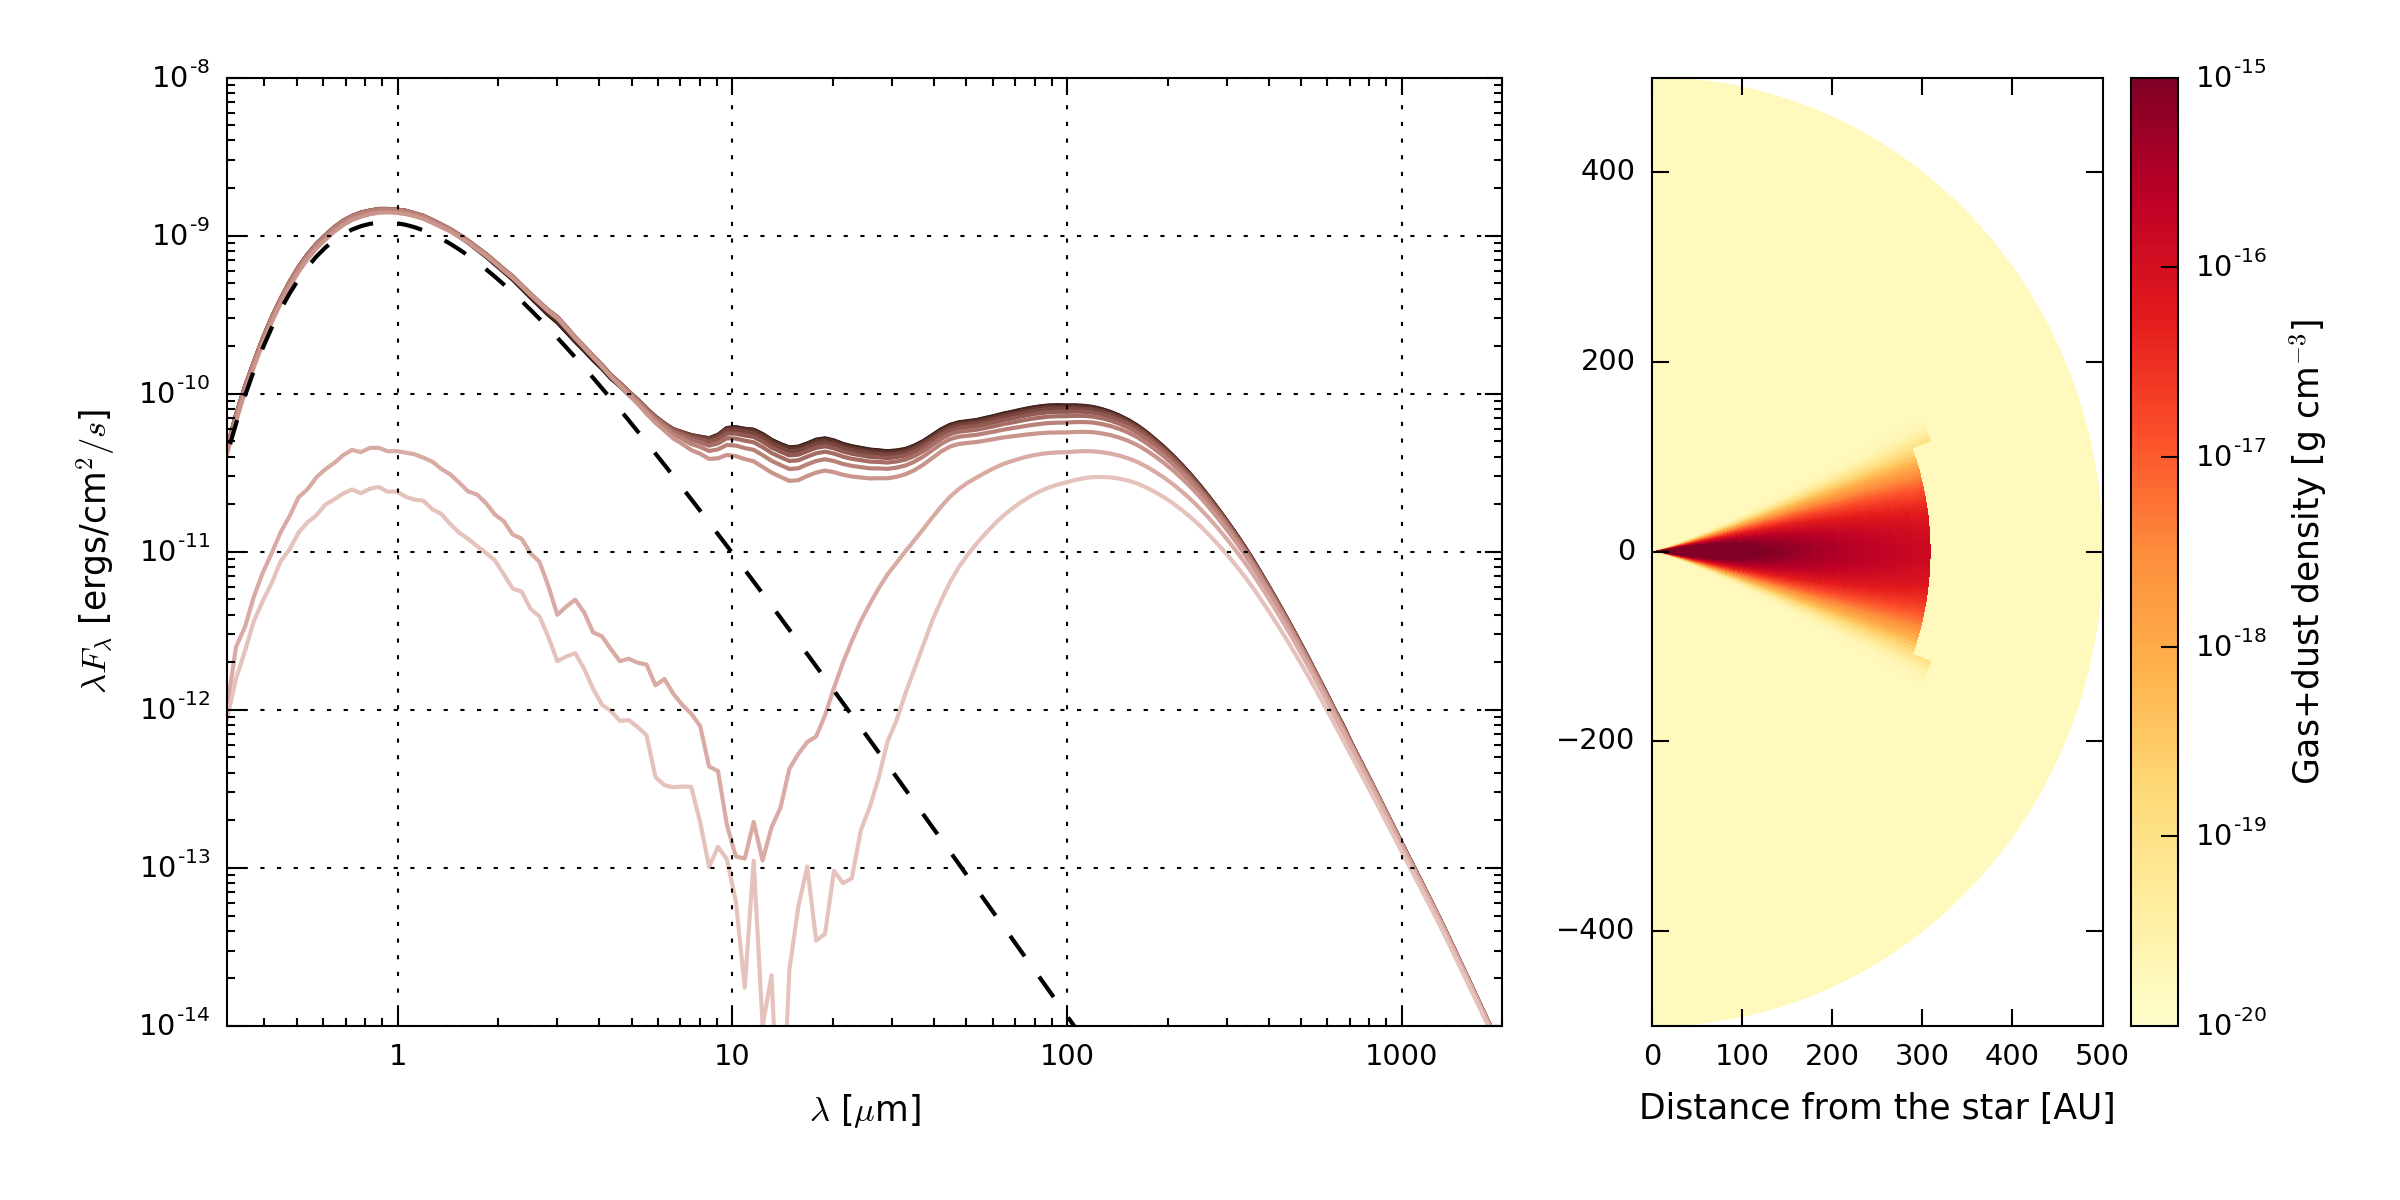
\includegraphics[width=\textwidth]{Figures/test_whitney_classII_nice.png} 
} \par\medskip
\subcaptionbox{Stage III.\label{subfig:StageIII}}{
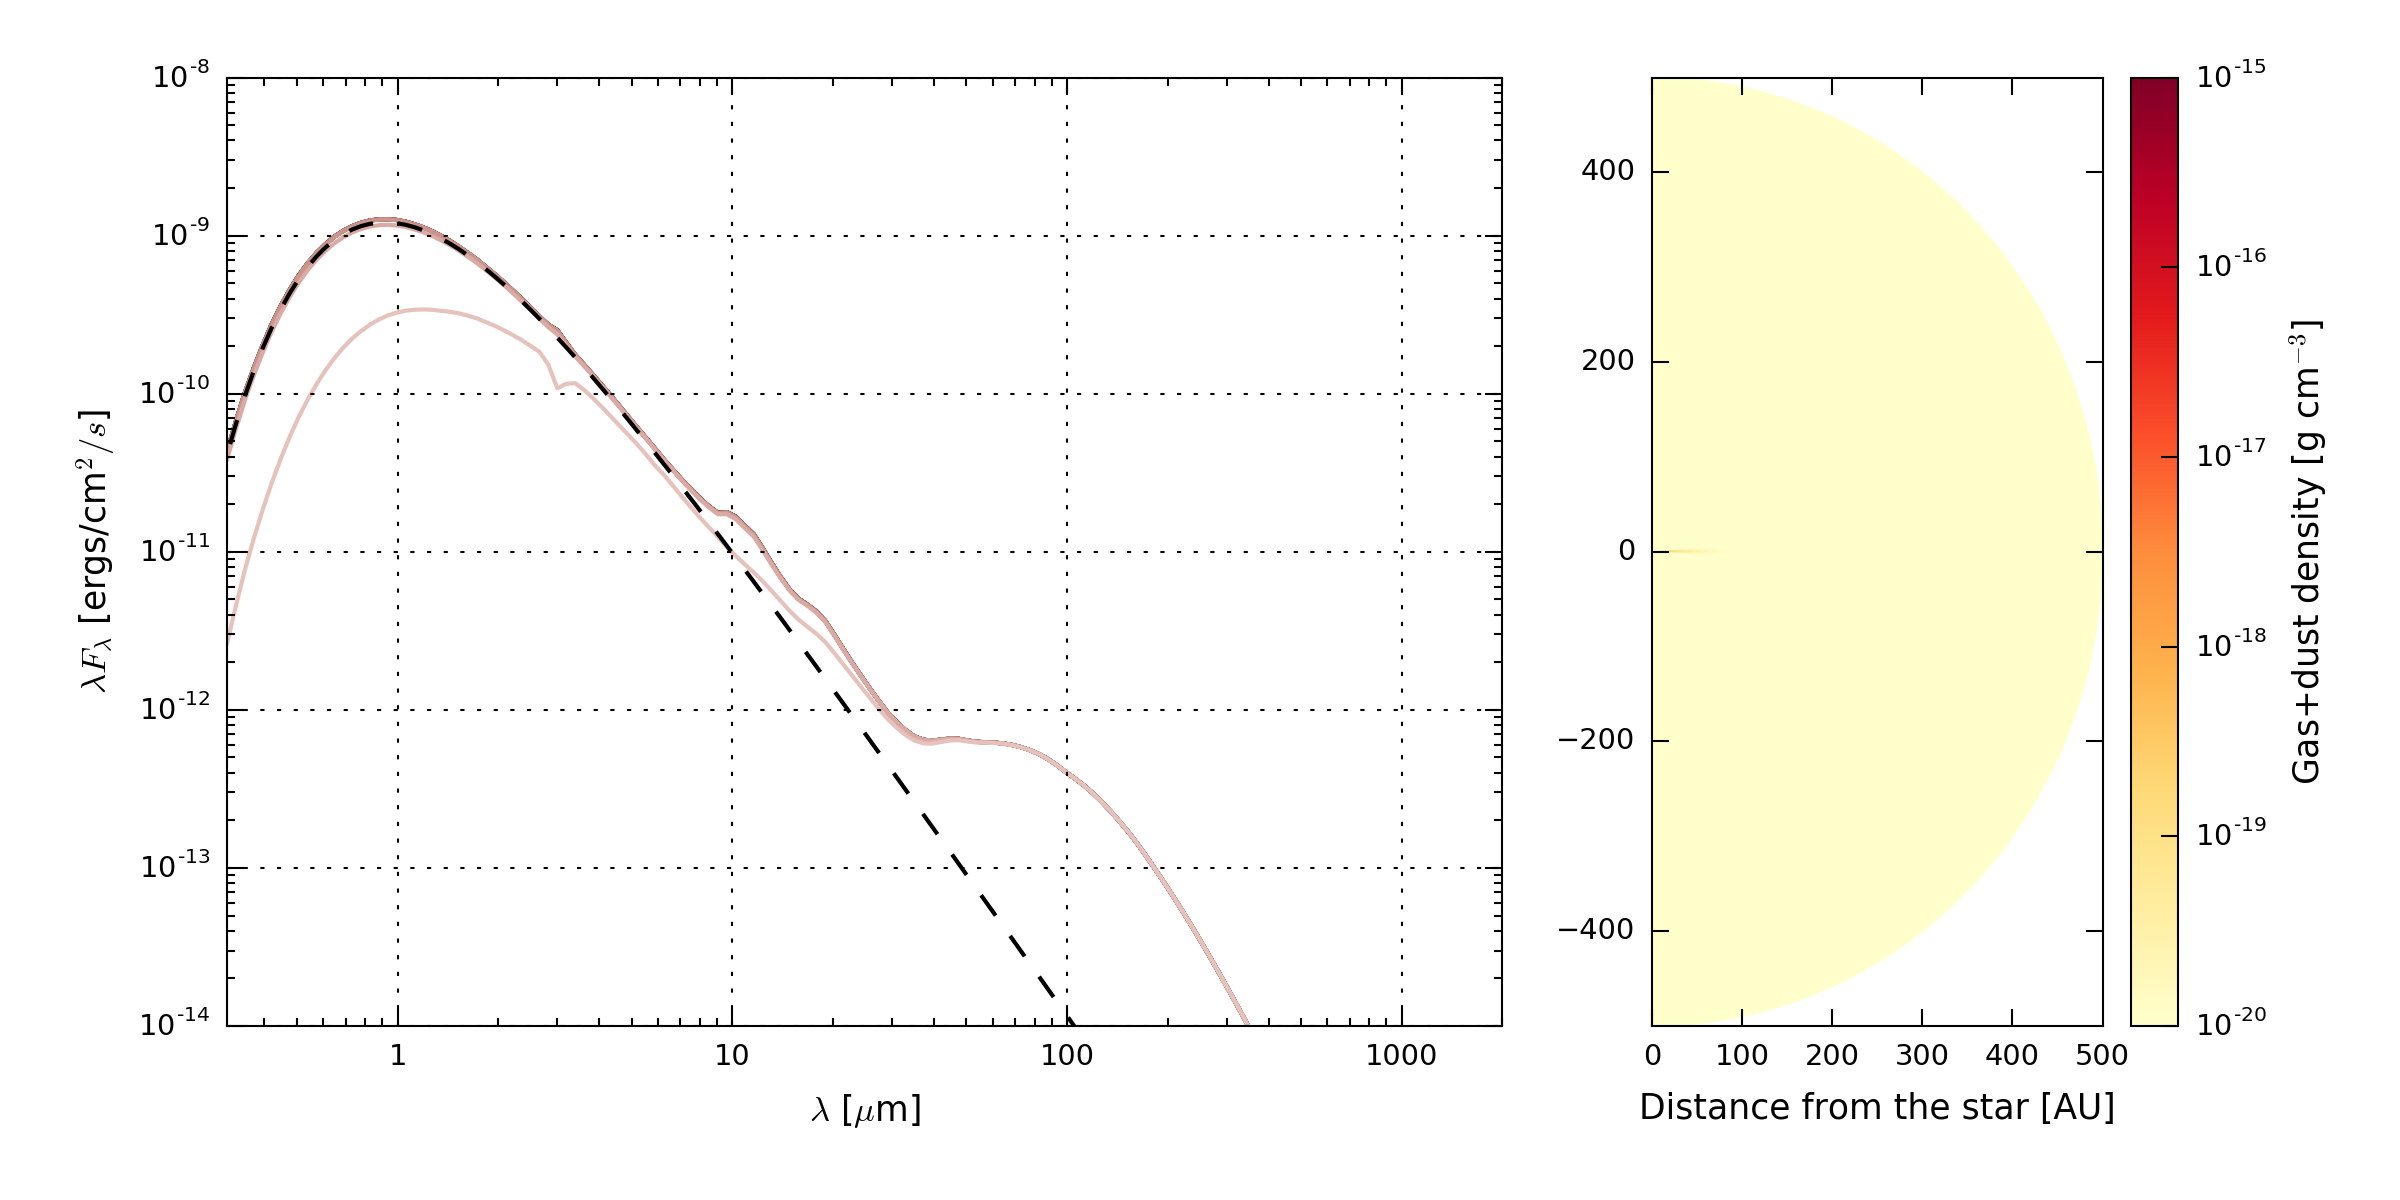
\includegraphics[width=\textwidth]{Figures/test_whitney_classIII_nice.png} 
}
\caption[Late evolution of YSOs]{Late evolution of YSOs.}
\label{fig:LateStages}
\end{center}
\end{figure}


\begin{itemize}
\item Class 0: Most the of short-wavelength ($<\SI{10}{\micro\meter}$) light is highly obscured by the dust in the massive envelope. Most of the emission is around \SI{100}{\micro\meter} and into the submillimeter/radio regimes. If there is a disk, it is very small. Some authors \citep{Dunham:2010bx} classify a source as Class 0 as long as the amount of the mass in the envelope is at least half the total mass.
\item Class I: Light scatters at short wavelength off the dust grains to give us a hint at the embedded object, but it still very obscured. The envelope's mass is lower, and the disk extends to larger distances. The typical spectral index $\alpha$ is positive.
\item Class II: The YSO is now a pre-main sequence star, with a spectral index $-1.5 < \alpha < 0$ a significant circumstellar disk. This is traditionally referred to as a classical T-Tauri star.
\item Class III: Still a pre-main sequence star, but most of the accretion has stopped, and $\alpha < -1.5$. The envelope has almost completely disappeared, and so has most of the disk.
\end{itemize}

An illustration of canonical spectral energy distributions (SED) and density structure is shown in Figs.~\ref{fig:EarlyStages,fig:LateStages} for the four main stages, with parameters taken in \citet{Whitney:2003kc}. On the left of each picture, the SED is the measurable quantity when the YSO is unresolved at all wavelengths. The challenge is to estimate the density structure (to the right) by measuring the SED. The different lines plotted in the SEDs are different inclination angles, highlighting the enormous impact of the viewing angle on the potential interpretation of these SEDs. The dashed line corresponds to the Planck function from the central source. These models were run using the Hyperion software \citep{Robitaille:2011fc} with "OH5" dust \citep{Ossenkopf:1994tq}, as discussed in more details in Section~\ref{subsec:dust}.

These SEDs are often characterized and classified with standard observational metrics, such as the bolometric temperature and luminosities \citep{Myers:1993en,Dunham:2010bx}:

\begin{align}
\Lbol &= 4\pi d^2\int_0^\infty\Snu d\nu,\\
\Tbol &= \num{1.25e-11} \frac{\int_0^\infty \nu\Snu d\nu}{\int_0^\infty \Snu d\nu}~\si{\kelvin},
\end{align}
%
where \Snu is the flux density in \si{\watt\per\raiseto{2}\meter\per\hertz}. 

\subsection{Mass accretion in clusters}


The discussion in the previous section represents a canonical view of how a single core collapses and forms a star. While it is convenient to assume that the original core forms a fixed reservoir of gas that will determine the star's final mass, it is likely too simplistic, since these YSOs are preferentially forming inside of clusters close to multiple other YSOs and sharing a dense, often turbulent environment \citep{Porras:2003kxa,Allen:2007wqa,Gutermuth:2009gca}. 

%Approximately 60\% of all stars are thought to form in clusters with 100 or more stars (\cite{Porras:2003p1395}; \cite{Allen:2007p1439}). These $>$100 star clusters have characteristic sizes of 2-4 parsecs with peak surface densities of 100-1,000 stars per square parsec and a typical median distance between nearest neighbor young stellar objects (YSOs) of 0.03 to 0.06 parsecs \citep{Gutermuth:2009p1325}.

The question of how stars acquire their final mass is key in studying star formation. Does dense gas fragment into isolated centers of collapse? Do young stars competitively accrete material from a surrounding common reservoir? Do gravitational interactions between forming young objects play a significant role in setting the final stellar mass function? Better observational understanding of these clusters is necessary to address these questions and to discriminate between the different models, as noted by \cite{Bonnell:2006ee}, \cite{Offner:2011ex} and \cite{Myers:2011fy}.

Given the typical stellar separations in clusters with fully formed young stellar objects and the typical densities of gas in these cores, \num{1000}'s of astronomical units (\si{\au}, \SI{1}{\parsec} = \SI{206265}{\au} - are the size scales over which forming stars must draw material to become 0.5-10 solar masses. Once the material is inside \SI{100}{\au}, it is strongly bound to the forming stellar system (which may be one or more stars) and its fate is determined. To give an idea of the possibilities for accreting material, Fig. \ref{fig:SFscenarios} sketches three scenarios for how stars could capture mass in the cluster environment: core collapse, competitive accretion, and collisional merging. In core collapse (CC) \citep[Fig.~\ref{scenarios:a},][]{McKee:2003gxa, Myers:2011fy}, the cluster's gas fragments into cores which collapse individually to form single, binary, or small multiple star systems; the available mass is defined by the original fragment. In competitive accretion (CA) \citep[Fig.~\ref{scenarios:b},][]{Bonnell:1997vta}, the initial core collapses but contains a small fraction of the star's final mass; additional mass is captured competitively with other forming stars from the surrounding dense core gas. In collisional merging (CM) \citep[Fig.~\ref{scenarios:c},][]{Bonnell:2002et}, the initial fragments interact gravitationally and form larger mass cores before and during the formation process. 

Are all these processes observed at once in star forming clusters? What conditions favor one versus the other, and why? Are these processes observed at different stages in the cluster's history?

Recent studies by \cite{Offner:2011ex} and \cite{Myers:2011p1338} compared protostar luminosity distributions with predictions of models based on these ideas. \cite{Offner:2011ex} suggest that both CC and CA could work if the star formation rate in the cluster increases with time; \citep{Myers:2011fy} finds that a CA-type model with additional Bondi accretion to produce massive stars works best. As highlighted at the end of the \cite{Offner:2011ex} paper, larger cluster samples and better data on massive stars are needed to improve the observational constraints on models.


%\paragraph{The Initial and Core Mass Functions}
%Initial mass function across multiple locations \citep{Myers:2014ct}: The IMF has similar properties of shape, mass scale, and high-mass slope among field stars, open clusters, and young clusters (Kroupa 2002, Chabrier 2005, Bastian et al. 2010).
%
%In the most widely-discussed explanation, an IMF distribution of masses arises as a cluster-forming clump fragments into condensations, or cores, due to self-gravity and turbulence. In such turbulent fragmentation models, the mass distribution of cores (CMF) is a mass-shifted version of the IMF (Padoan \& Nordlund 2002, Hennebelle \& Chabrier 2008, Hennebelle \& Chabrier 2009, Hopkins 2012), matching observational studies of cores in nearby star-forming regions (Motte et al. 1998, Alves et al. 2007, Konyves et al. 2010)
%
%\citep{Myers:2014ct} has all I need here to describe the IMF and CMF
%
%Describe the various theories of SF in clusters. 



\begin{figure}[ht!]
\begin{center}
\begin{subfigure}[b]{0.3\textwidth}
\centering

\includegraphics[width=0.98\textwidth]{Figures/CC.png} 
\caption{}
\label{subfig:scenarios:a}
\end{subfigure}
\begin{subfigure}[b]{0.3\textwidth}
\centering

\includegraphics[width=0.98\textwidth]{Figures/CA.png} 
\caption{}
\label{subfig:scenarios:b}
\end{subfigure}
\begin{subfigure}[b]{0.3\textwidth}
\centering
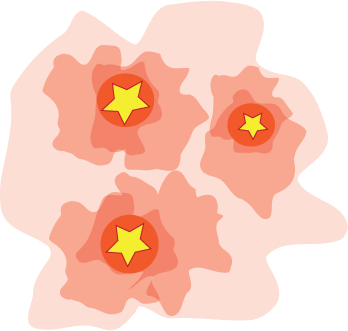
\includegraphics[width=0.98\textwidth]{Figures/Coalescence.png} 
\caption{}
\label{subfig:scenarios:c}
\end{subfigure}
\caption[Scenarios of clustered star formation]{Three scenarios of clustered star formation. Darker colors indicate higher densities.}
\label{fig:SFscenarios}
\end{center}
\end{figure}



%\subsubsection{Outstanding scientific questions}
%Examples: \citep{Hennebelle:2012dk} \citep{Kennicutt:2012ey}
%Ex: WHERE DO THE INEFFICIENCIES COME FROM?
%
%Luminosity problem \citep{McKee:2007bd}
%Angular momentum problem and magnetic flux problem  \citep{McKee:2007bd}
%How the mass-to-flux ratio increases so dramatically during star formation is one of the classic problems of star formation (Mestel \& Spitzer 1956). 

\section{Dust as a tracer of star formation}
\label{subsec:dust}

Despite being a small component by mass, interstellar dust is an important component of galaxies. Dust grains are heated up by absorbing the short wavelength emission from stars and re-radiate in the thermal infrared, accounting for $\sim 30\%$ of the total luminosity of the galaxy \citep{Mathis:1990jk}. 

Observationally, dust plays perhaps the most important role when it comes to studying star formation. It usually is assumed that dust is well mixed with the gas, which makes it an excellent tracer of the gravitational well and mass distribution in YSOs. Because H$_2$ and He molecules have very few spectral signatures, they are difficult to observe and study directly. Dust grains block UV and visible star light and emit continuum far-IR radiation, opening a large region of the electromagnetic spectrum for astronomers to study the properties of star formation. Alternative tools to study star formation are dedicated to observing spectral lines of the molecular compounds of the ISM such as CO and other dense gas tracers, a prospect that limits the study to the most dense regions since these compounds typically freeze out onto the surface of dust grains for sufficiently high densities [REF?]%and requires more assumptions to link the abundance of these compounds to the more massive neutral H$_2$ and He gas.


\subsection{Dust populations and properties}


Perhaps the first understanding of the composition of dust grains in the ISM was described by \cite{Mathis:1977hp}, where they studied the absorption spectrum of the diffuse ISM, and found that the measurements were appropriately fitted with a dust grain composition of silicates and small graphite particles \citep{Stecher:1965eq}. They were able to fit the observed extinction curve with canonical grain-size distribution, typically $n(a) \propto a^{-3.5}$, where $a$ is the grain size (assuming spherical grains) and $n(a)$ corresponds to the number of grains of sizes $<a$. This assumes low and high cutoffs for the grain sizes, typically \SI{50}{\angstrom} and \SI{0.25}{\micro\meter}, respectively.

This grain-size distribution model was later on enhanced by \cite{Cardelli:1989dp} to account for the difference in interstellar extinctions (hence size distributions) across different galactic lines of sight. These authors were able to successfully parameterize this size distribution using a single parameter, $R_V$, which is the ratio of the total extinction $A(V)$ to selective extinction\footnote{Extinction and colors are expressed in magnitudes} (or color) $E(B-V) = A(B) - A(V)$. Smooth distributions of sizes of graphite and silicate grains between the less dense regions of the ISM, where $R_V = 3.1$, and the dense clusters, where $R_V = 5.3$ \citep{Kim:1994iu}. 

Observations in the thermal infrared from space telescopes have detected strong absorption lines at \SI{9.7}{\micro\meter} and \SI{18}{\micro\meter} which are attributed to stretching mode of Si-O and bending mode of O-Si-O, confirming the presence of silicates in dust compositions \citep{Weingartner:2001du}. Other emission features at 3.3, 6.2, 7.7, 8.6, and \SI{11.3}{\micro\meter} \citep{Sellgren:1994vz} were attributed to bending and stretching modes of polycyclic aromatic hydrocarbons \citep[PAH, see][]{Gillett:1973bh,Allamandola:1985cf}, which are complex, planar organic molecules.
 
A consolidated model matching all-sky measurements by instruments on the COBE space observatory confirms the composition of amorphous silicates and carbonaceous grains with sizes ranging from large grains ($\approx\SI{1}{\micro\meter}$) down to tens of atoms \citep{Li:2001gk}, where the larger carbonaceous grains have graphitic properties and the smaller population have PAH-like properties.


[Molecular hydrogen is believed to form by recombination on the surface of dust grains [hollenbach and salpeter 1971, and are only able to survive from UV photodissociation within these obscured clouds.]




Knowing the dust composition and size distribution of grains is important to properly predict its observational behavior and relate it to the physical quantities of interest, since the goal of the exercise is to use dust as a tracer of star-forming mechanisms. A given dust model needs to provide several key quantities that can be used in radiative transfer modeling (see Section~\ref{subsubsec:radiative}), such as the albedo, the scattering function, and the opacity.

In the very cold regions surrounding a YSO, where the dust temperature typically never exceeds a few tens of \si{\kelvin}, it is expected that these dust grains are covered by a mantel of ices which can dramatically change their radiative properties, especially at short wavelengths. 

\subsection{Basics of dust extinction}

Dust grains are responsible for the extinction within molecular clouds, inside of clusters, and also within each YSO; although these various extinctions could originate in different types of grain populations. The typical representation of this extinction uses the ratio of observed over expected flux, measured in V-band: $\Av \equiv A(V) = 2.5\log(\Fnu^\textrm{obs}/\Fnu)$. The extinction, $A(\lambda)$, is a function of wavelength and is expressed in magnitudes. An alternative representation is to consider the extinction as being caused by an optical depth $\tau_\ext$ such as $\exp(-\tau_\ext) = \Fnu^\textrm{obs}/\Fnu$. We have the equivalence $A(\lambda) = \num{1.086}\tau_\ext(\lambda)$.

At sufficiently long wavelength, dust opacity models can usually be represented by a simple power-law, $\Knu = \kappa_0(\nu/\nu_0)^\beta$, with the index $\beta$ depending on the specifics of the dust model. The opacity $\Knu$ is expressed in \si{\raiseto{2}\centi\meter\per\gram}, and can be interpreted as a extinction cross-section per unit mass. Most dust models assume a 1:100 dust-to-gas ratio, and derive opacities per unit {gas+dust} mass, instead of just dust mass. From a radiative transfer perspective, the observed specific intensity from a thermal source $\Bnu(T)$ in the optically thin regime is $I_\nu = \tau_\nu \Bnu(T)$, where the optical depth is $\tau_\nu = \Knu\int{\rho_\dust dl}$. $\rho$ is the density and the integral is calculated along the line of sight to the source. %Note that the optical depth can also be expressed in terms of the extinction cross-section \Cext~as $\Knu = \Cext(\nu) / m_\dust$, where $m_\dust$ corresponds to the mass of a dust grain.

A measure of the intensity from a source can thus lead to an approximation of the total mass within a primary beam, for a given dust grain model. For a source with a measured sub-millimeter flux density $S_\nu$, in the optically thin regime we can write $S_\nu=\tau_\nu\Bnu(T)\Omega$, where $\Omega$ is the solid angle of the source, $\Omega = A/d^2$, with $A$ the area of the source and $d$ its distance. We obtain a measure of the mass by writing $M\approx A\int{\rho dl}$, to obtain \citep{Shirley:2000gh}:
\begin{equation}
M = \frac{S_\nu d^2}{B_\nu(T_\dust)\Knu},
\end{equation}
with a dust temperature is usually taken to be between 10 to \SI{20}{\kelvin}. 

With only near- to far-IR wavelengths observations, however, it is more difficult to estimate the dust mass, because the system is usually not in the optically thin regime and very dependent on the local geometry and viewing angle. To use these observations, which are interesting because they naturally are at higher resolution than single-dish submillimeter data, detailed radiative transfer models are usually required (Section~\ref{subsubsec:radiative}).


Dust grains can either scatter or absorb photons, and both of these processes have their own frequency-dependent efficiency. Large grains are usually considered in local thermal equilibrium (LTE), in which case the thermal emission balances out the absorption. However, small grains ($<\SI{50}{\angstrom}$) can be subject to stochastic heating, where single photons can heat up the grains to much higher temperatures for very short amounts ot time. Scattering mechanisms can be much more complicated to represent, as they usually involve a scattering phase function, describing the deflection angle of incident photons (which also depends on wavelength). Most models show that dust grains are preferentially forward-scattering [CITE Draine?]. The scattering properties of the dust model exclusively influence the short-wavelength emission, while the absorption properties influence all wavelengths. 

%Talk about dust properties in the galaxy: \citep{Collaboration:2014dz} Using
%Also maybe mention papers by Dale etc DIRBE/COBE
%
%A large number of dust models exist (see Section~\ref{subsubsec:radiative})
%
%In clusters and cores, it is likely that grains are covered with a layer of ice which could dramatically influence their radiative transfer properties

\subsection{Radiative transfer modeling}
\label{subsubsec:radiative}

Several radiative transfer codes exist in the literature, and we have explored a few of them. We opted for a recently-developed package called Hyperion \citep{Robitaille:2011fc}, which is a Python interface to a 3D Monte-Carlo code by \citet{Whitney:2013cw}. The code is versatile, parallelized, can accept different dust models and can generate various types of geometries and density grids.

Hyperion functions in two steps. After choosing a discrete grid to represent a density model and adding energy sources, the temperature structure of the dust is calculated by propagating photon packets and determining the dust LTE temperature in each cell. Multiple iterations of this process are usually required to converge to a decent thermal structure.

Once the dust temperature is known, the dust becomes a source of thermal radiation. This type of radiation is modeled using ray tracing, which provides a very good signal-to-noise ratio (\SNR). The light from the central source which was not absorbed, however, needs to be propagated and scattered off the dust grains, for example using a method called peeling-off \citep{YusefZadeh:1984ff}. For non-isotropic scattering, this process has relatively low \SNR, hence requires a lot of photons packets to function properly. While there are future plans to implement raytracing for scattering \citep{Robitaille:2011fc}, we are currently forced to wait long times for simulating YSOs with massive envelopes because of this problem.

[Put models of YSOs with different masses here.]

These models usually present a large amount of degeneracies, especially when the entire range of wavelengths is not covered, as it is the case for most astronomical sources. For example, an SED will look very different depending on the viewing angle. If we see down the throat of the cavity, the short-wavelength light from the central source will not exhibit a lot of extinction. If we observe this same source through the disk and envelope, these same wavelengths will show a lot of extinction. The short wavelength, up to the peak of the SED, are very geometry-dependent and highly degenerate parameters.

This realization helped us target our work using this code. Others \citep[e.g][]{Robitaille:2006cb} have produced standardized grids of pre-computed models which randomly sample a very large number of source geometry parameters. These grids are routinely used by the community to fit a set of unresolved SED measurements at discrete wavelengths. However, most often the scatter in the parameters for the few best fit models prevents from drawing meaningful conclusions on the observations. 

[Example?]
%For example, in a Class 0 or I YSO, the disk geometry and mass has a very insignificant impact on the resulting SED. [Put a model of the SED with and without disk?]

One of the key challenges of using this code is to determine which dust models to use. For this work, we choose to use exclusively OH5 dust \citep{Ossenkopf:1994tq}, which represents grains with an ice mantle which are the result of a coagulation phase of an initial distribution of grain sizes following $n\propto a^{-3/2}$. This model was found to accurately represent some grain distribution in the ISM [NEED CITATION, CHECK OUT TRACY'S PAPER].

\subsection{Observing star formation}

In the past decade, space-based infrared observatories such as \Spitzer\ and \Herschel\ have really allowed the beginning of the detailed study of dust around forming stars, by sampling the SEDs in key spectral regions, such as the PAH region (with the IRAC instrument on \Spitzer), the mid-infrared (with the MIPS instrument, especially its \SI{24}{\micro\meter} channel), and the far-IR (with the PACS instrument on \Herschel). 

However, these observatories lack the required angular resolution to observe the key physics of star formation in dense clusters in the key wavelength region between \SI{30}{\micro\meter} and \SI{200}{\micro\meter}. For a diffraction-limited single aperture telescope, the angular resolution and spatial resolutions $R_\theta$ and $R_\textrm{linear}$ are:
\begin{align}
R_\theta &= \ang{;;17.6}\left(\frac{\lambda}{\SI{70}{\micro\meter}}\right)\left(\frac{D}{\SI{1}{\meter}}\right)^{-1}, \\
R_\textrm{linear} &= \SI{0.04}{\parsec}\left(\frac{d}{\SI{500}{\parsec}}\right)\left(\frac{\lambda}{\SI{70}{\micro\meter}}\right)\left(\frac{D}{\SI{1}{\meter}}\right)^{-1},
\end{align}
which shows that even with \Herschel and its \SI{3.5}{\meter} primary mirror and its \SI{70}{\micro\meter} channel, we can barely resolve clustered YSOs (typical separations of a few hundredths of \si{\parsec}), let alone study their structure in detail. 

To further complicate the problem, most space observatories are tailored for very sensitive observations, so the brightest regions of clusters often cause saturation issues due to a lack of dynamic range. These two issues have continually prevented us from gathering a good picture of the physics in these dense and important regions of stellar birth.

[Image that shows the saturation/lack of resolution]

[Talk about SOFIA]
%\subsubsection{Observing facilities}
%
%Introduction notes: [DELETE THIS]
%\begin{itemize}
%\item \citep{Kennicutt:2012ey} Maybe start with a description of the ISM
%\item \citep{Terebey:1984hi} Basics of infall; 
%It is well understood how self-gravity can concentrate gas in the presence of magnetic fields, turbulence, rotation, and thermal pressure, leading to protostar formation and accretion ( McKee \& Ostriker 2007; Adams \& Shu 2007; Ballesteros-Paredes et al. 2007)
%\item \citep{Adams:1987gy} Spectral evolution of young stellar objects; describe classes of stellar objects, using models and make sure to include size scales; YSO vs protostar
%\item Need to mention something about star formation efficiency
%\item Need to mention something about outflows and feedback \citep{Maury:2009co}
%\item \citep{Larson:1994cj} Molecular cloud characteristics; maybe a good start for text | Give definition of cloud (gravitationally bound in the Virial sense), in terms of number of candidates and stellar mass density (Lada 2003)
%\item \citep{Myers:2009fv} It is widely accepted that most stars form in concentrations of dense gas (Beichman et al. 1986), and that such young stars are most frequently found in groups and clusters in molecular clouds (Lada \& Lada 2003). It is less clear how the mass of a protostar is related to the mass of the dense core where it forms.
%In one view, a core is essentially a fixed-mass reservoir of gas, which contributes a significant fraction of its initial mass to its protostar. Then core and protostar masses are proportional, and their mass distributions have the same shape (Motte et al. 1998; Alves et al. 2007). Many authors have suggested ways to form a mass distribution of cores which resembles the IMF, particularly from processes of turbulent fragmentation (Hennebelle \& Chabrier 2008 and references therein).
%In another view, a core is the densest part of a more extended distribution of gas, with no physical barrier to accretion (Shu 1977; Myers \& Fuller 1992; Caselli \& Myers 1995; McKee \& Tan 2003). Protostars originate in cores, but their masses do not correlate (Bonnell et al. 1998; Bate \& Bonnell 2005), or their correlation depends on fragmentation and core definition (Swift \& Williams 2008), or on the range of gas dispersal times (Myers 2008, hereafter Paper 1). Alternately, their correlation may be coincidental rather than genetic (Hatchell \& Fuller 2008).
%\item \citep{McKee:2010iw} Protostellar mass function
%\item \citep{Bonnell:1997vta} Accretion in small clusters
%\item \citep{Evans:1999gz} Review of physical conditions of star formation, also a good place to start
%\item \citep{Myers:2011fy} These results suggest that a simple model is needed for the dense parts of clusters, where protostars start accreting in condensations resembling dense cores, where they can also gain mass from the core environment, where their accretion durations are specified, and where protostar mass is not tied to the gravitational collapse of an isolated initial condensation. | This comparison favors the core–clump model over the isolated core model for star formation in embedded clusters. It suggests that initial core structure need not set protostar mass, and that massive stars are clump-fed.
%\item Clusters are laboratories for studying a wide range of astrophysical phenomena; stars of large range of masses which are formed roughly simultaneously (Lada 2003), can understand stellar evolution theories; 
%\item \citep{Lada:2003il} Cluster formation within molecular clouds: Because a cluster is held together by the mutual gravitational attraction of its individual members, its evolution is determined by Newton's laws of motion and gravity; |
%Stars form in dense gas; therefore, it is not surprising that a high fraction of all stars form in highly localized rich clusters because most of a cloud’s dense gas is contained in its localized massive cores.; |
%This would suggest that there is a direct mapping of clump mass to stellar mass and that the substructure of cluster-forming cores reflects the initial conditions of the star-formation process in dense cores. |
%The structure of an embedded cluster is of great interest since it likely possesses the imprint of the physical process responsible for its creation. In particular, structure in the youngest embedded clusters reflects the underlying structure in the dense molecular gas from which they formed. | A fundamental consequence of the theory of stellar structure and evolution is that, once formed, the subsequent life history of a star is essentially predetermined by one parameter, its birth mass
%\item \citep{Bate:2003cv} Evolution of clusters (dynamics, showing simulations and such); same as \citep{Bonnell:2003iw}; realte to potentially having multiple generations of stars within the same cluster; \citep{Allen:2007wqa}
%\item \citep{Mathis:1990jk} Pioneering paper on the interstellar extinction by dust
%\item \citep{Weingartner:2001du} Paper on dust populations
%\item \citep{Li:2001gk} Very small grain population and non-LTE heating
%\item \citep{Compiegne:2010kk} Large surveys, PAHs, VSG, etc
%\item \citep{Bastian:2010ig} Big picture: importance to universal IMF
%\item \citep{Kennicutt:2012ey} The Challenge of Spatially Resolved Star-Formation Rates in Galaxies
%\item \citep{Hennebelle:2012dk} Observational issues: 
%
%\end{itemize}
%


%How do stars accrete their material in dense, clustered environments? Multiple theories have been put forth to explain the forces at play in these important regions of stellar birth \citep[e.g.][]{Bonnell:1997vta, McKee:2003gxa}. Pivotal differences in the theories center around what drives the parsec-scale dense cloud to form many stars and how the forming stars acquire their mass. Does dense gas fragment into isolated centers of collapse? Are turbulent motions in the gas driving creation of super-critical cores? Do young stars competitively accrete material from a surrounding common reservoir? Do gravitational interactions between forming young objects play a significant role in setting the final stellar mass function? Better observational understanding of these clusters is necessary to address these questions and to discriminate between the different models, as noted by \cite{Bonnell:2006ee}, \cite{Offner:2011ex} and \cite{Myers:2011fy}.
%
%\textbf{The primary goal of the proposed science plan is to understand how stars accrete material on the scales of 100's to 1,000's of AUs in forming cluster cores}. Given the typical stellar separations in clusters with fully formed young stellar objects (YSO) and the typical densities of gas in these cores, 1,000's of AUs are the size scales over which forming stars must draw material to become 0.5-10 solar masses. Once the material is inside 100 AU, it is strongly bound to the forming stellar system (which may be one or more stars) and its fate is determined. To give an idea of the possibilities for accreting material, Fig. \ref{fig:SFscenarios} sketches three scenarios for how stars could capture mass in the cluster environment: core collapse, competitive accretion, and collisional merging. In core collapse \citep[Fig.~\ref{scenarios:a},][]{McKee:2003gxa, Myers:2011fy}, the cluster's gas fragments into cores which collapse individually to form single, binary, or small multiple star systems; the available mass is defined by the original fragment. In competitive accretion \citep[Fig.~\ref{scenarios:b},][]{Bonnell:1997vta}, the initial core collapses but contains a small fraction of the star's final mass; additional mass is captured competitively with other forming stars from the surrounding dense core gas. In collisional merging \citep[Fig.~\ref{scenarios:c},][]{Bonnell:2002et}, the initial fragments interact gravitationally and form larger mass cores before and during the formation process. 
%
%Are all these processes observed at once in star forming clusters? What conditions favor one versus the other, and why? Are these processes observed at different stages in the cluster's history? These questions need more observational data to be answered. \textbf{We propose to gather information about the gravitational potential within the cluster, the distribution of the turbulence, and the gas densities} \citep{Bonnell:2006ee}. This will advance the problem to the next stage and help answer some of these questions.
%


%\subsection{The physics of star formation}
%
%In here, describe the basics of star formation; include state-of-the art dynamical modeling, radiative transfer modeling, SED fitting, etc.
%
%\subsubsection{Dust populations}
%
%About how to estimate the mass
%
%\subsubsection{Geometry and model degeneracies}
%
%\subsubsection{Foreground extinction}
%
%\subsection{Clustered environments}
%
%\subsubsection{Observational challenges}
%
%Surveys vs pointed observations; show why BETTII is important using IRAS20050's example;
%
%\subsubsection{Observing facilities}
%
%Spitzer, Herschel, SOFIA; radio interferometers;

